\documentclass[12pt,a4paper, margin=1in]{article}
\usepackage{fullpage}
\usepackage{amsfonts, amsmath, pifont}
\usepackage{amsthm}
\usepackage{amsmath}
\usepackage{graphicx}
\usepackage{geometry}
\graphicspath{"."}
\geometry{
a4paper,
% total={210mm,297mm},
left=12mm,
right=12mm,
top=10mm,
bottom=10mm,
}

\author{
Ahmet Eren Çolak\\
\texttt{e2587921@ceng.metu.edu.tr}
}
\title{\textbf{CENG 499 - Introduction to Machine Learning} \\
Homework 1 - Part 3}
\begin{document}
\maketitle

\noindent\rule{19cm}{1.2pt}
\newcommand\ddfrac[2]{\frac{\displaystyle #1}{\displaystyle #2}}

\bigskip \bigskip

Throughout the process, 10 different configurations of hyperparameters are trained which includes combinations of hidden layer count, neuron counts in layers, activation function, learning rate and epoch. 
All of these configurations are trained with stochastic gradient descent. 

\bigskip

\begin{table}[h]
    \begin{tabular}{|c|c|c|c|c|c|c|}
    \hline
    \textbf{ID} & \textbf{\begin{tabular}[c]{@{}c@{}}Hidden \\ Layers\end{tabular}} & \textbf{\begin{tabular}[c]{@{}c@{}}Hidden Layer 1\\ Neuron Count\end{tabular}} & \textbf{\begin{tabular}[c]{@{}c@{}}Hidden Layer 2\\ Neuron Count\end{tabular}} & \textbf{\begin{tabular}[c]{@{}c@{}}Activation\\ Function\end{tabular}} & \textbf{\begin{tabular}[c]{@{}c@{}}Learning \\ Rate\end{tabular}} & \textbf{Epochs} \\ \hline
    1           & 1                                                                 & 16                                                                             & -                                                                              & Sigmoid                                                                & 0.001                                                             & 5               \\ \hline
    2           & 1                                                                 & 32                                                                             & -                                                                              & Sigmoid                                                                & 0.001                                                             & 5               \\ \hline
    3           & 1                                                                 & 16                                                                             & -                                                                              & LeakyReLu                                                              & 0.001                                                             & 5               \\ \hline
    4           & 1                                                                 & 16                                                                             & -                                                                              & Tanh                                                                   & 0.001                                                             & 5               \\ \hline
    5           & 1                                                                 & 32                                                                             & -                                                                              & LeakyReLu                                                              & 0.001                                                             & 5               \\ \hline
    6           & 1                                                                 & 16                                                                             & -                                                                              & Sigmoid                                                                & 0.001                                                             & 8               \\ \hline
    7           & 1                                                                 & 16                                                                             & -                                                                              & Sigmoid                                                                & 0.01                                                              & 5               \\ \hline
    8           & 2                                                                 & 16                                                                             & 16                                                                             & Sigmoid                                                                & 0.001                                                             & 5               \\ \hline
    9           & 2                                                                 & 32                                                                             & 32                                                                             & Sigmoid                                                                & 0.01                                                              & 5               \\ \hline
    10          & 2                                                                 & 32                                                                             & 32                                                                             & Sigmoid                                                                & 0.001                                                             & 8               \\ \hline
    \end{tabular}
    \centering
    \caption{Hyperparameter configurations}
\end{table}

\bigskip

I created configurations 1,3 and 4 to determine the best performing activation function among sigmoid, tanh and leaky relu. Configurations 1,2 and 3,5 tests which count of neuron performs better. 6 and 1 configurations help with determining when to stop training the model. Configurations 8, 9 and 10 determines which hidden layer count and neuron counts are better.
Configurations 7 and 1 test the impact of learning rate on performance.
\pagebreak

Below table shows the confidence intervals of test accuracy for each hyperparameter configuration.

\begin{figure}[h]
    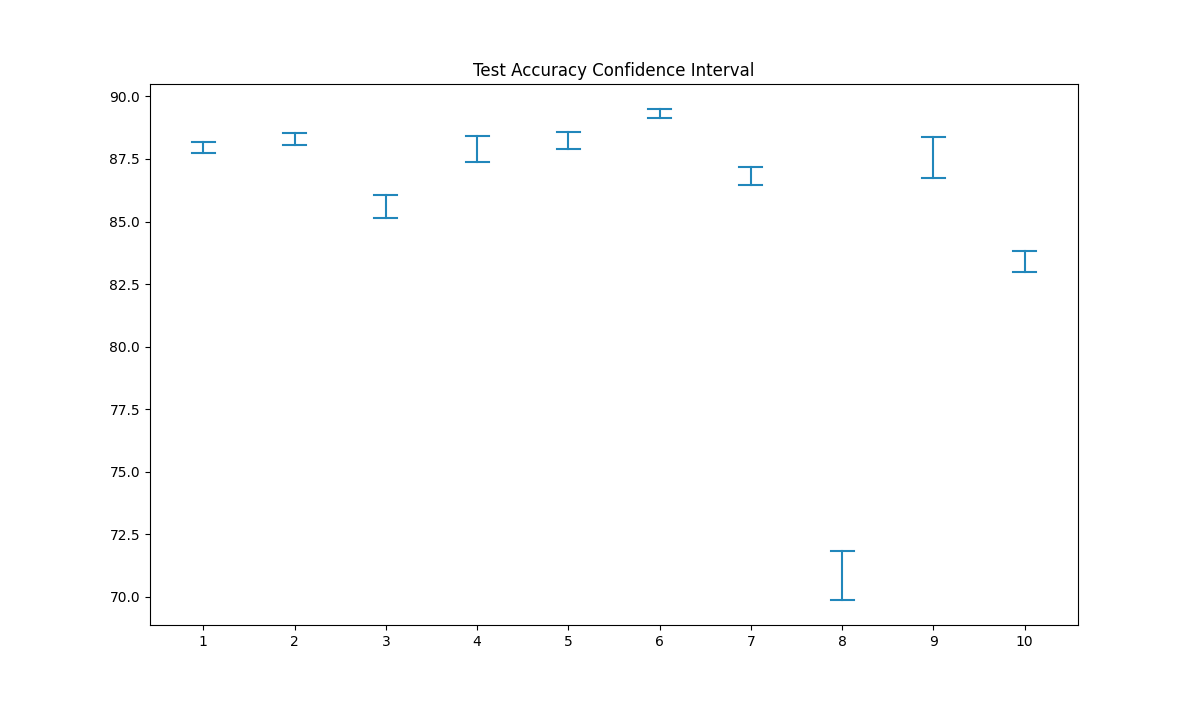
\includegraphics[scale=0.65]{srm_plot.png}
    \centering
    \caption{Confidence intervals}
\end{figure}
\bigskip

The first thing that draws attention is the poor performance of the 8th configuration which has 2 hidden layers and 16 neurons at each layer with learning rate 0.001. Increasing the hidden layers suprisingly reduced the performance. On the other hand increasing the neuron counts and lowering the learning rate increased the accuracy as it can be seen in the 9th configuration.
Again decreasing the learning rate back to 0.001 lowered performance as in the 10th configuration, in despite of higher epochs. 
In general models with 2 hidden layers performed worse than others which might be because of insufficient training. 

Another noticable thing is the poorer performance of leaky relu with 16 neurons in the hidden layer. Other than that tanh and sigmoid performed similarly.

Overall, the best performing configuration is the 6th one which has 16 neurons in a single hidden layer with learning rate 0.001, sigmoid activation function and 8 epochs.
I can conclude that 5 epochs is not sufficient and most configurations underfits
.
\section*{Answers}
\subsection*{a}
I tried two different configurations 1 and 6, one is trained till 8 epochs and the other one is trained till 5 epochs. Comparison of these two configurations may tell me whether i am overfitting or underfitting and when to stop.

\subsection*{b}
If test error is increasing or stays at the same level for a while, it means that model starts to overfit.

\subsection*{c}
If we check validation error at each iteration, then we can know that we should stop if validation error is increasing.

\subsection*{d}
In models with single layer, 0.001 seems the best one.

\subsection*{e}
Leaky relu performs definitely worse than the sigmoid and tanh functions. However tanh and sigmoid performs similarly.

\subsection*{f}
Smaller learning rates are more sensitive to find a local minima but they are costly in terms of efficiency

\subsection*{g}
Although big learning rates are more efficient, they may miss local minimums. 

\subsection*{h}
Stochastic gradient descent is appropriate for large datasets, since large samples are going to introduce more variety it may lead to better performance.
Downside of this approach may be the parallelization difficulties.

\subsection*{i}
Without data normalization, derivatives of activation functions are going to be same for most of the values which is undesired for updating parameters. Because for large and small values tanh and sigmoid functions rapidly converge. 

\end{document}